This is the node tree for searching algorithm. Different colors indicate different level of searching steps. %\vskip 0.5cm


\tikzset{
	level/.style={sibling distance=35mm/#1},
	treenode/.style={align=center,inner sep=0pt},
	% Black nodes
	node_black/.style={treenode,circle,black,draw=black,very thick,text width=0.5cm},
	% Red nodes
	node_red/.style={treenode,circle,red,draw=red,very thick,text width=0.5cm},
	% Blue nodes
	node_blue/.style={treenode,circle,blue,draw=blue,very thick,text width=0.5cm},
	% Nil nodes
	node_nil/.style={treenode,rectangle,fill=black,minimum width=0.3cm,minimum height=0.3cm}
}
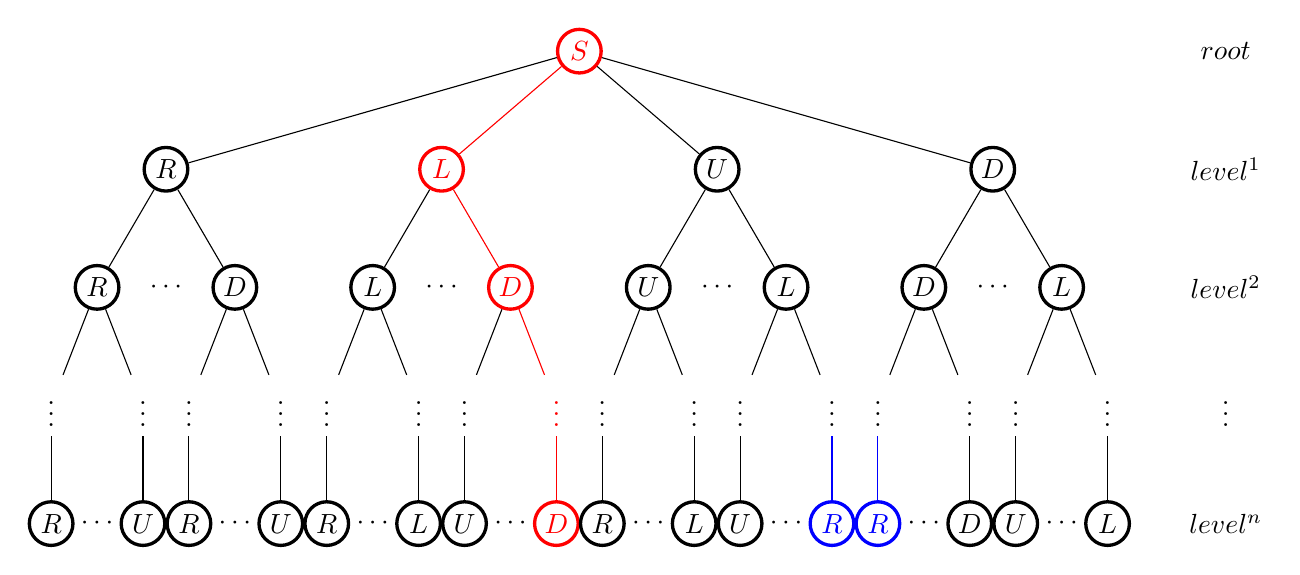
\begin{tikzpicture}
\node[node_red] (z){$S$}
  child {node[node_black] (a) {$R$}								%%% Right
    child[black] {node[node_black]  (b) {$R$}
      child {node (b1) {$\vdots$}
       child {node[node_black] (b11) {$R$}}
      }
      child {node (b2) {$\vdots$}
       child {node[node_black] (b12) {$U$}}
      }
    }
    child[black] {node[node_black] (g) {$D$}
      child {node (g1) {$\vdots$}
       child {node[node_black] (g11) {$R$}}
      }
      child {node (g2) {$\vdots$}
       child {node[node_black] (g12) {$U$}}
      }
    }
  }
   child[red] {node[node_red] (d) {$L$}                    %%%% LEft - the shortest parth
      child[black] {node[node_black]  (e) {$L$}
        child {node (e1) {$\vdots$}
         child {node[node_black] (e11) {$R$}}
        }
        child {node (e2) {$\vdots$}
         child {node[node_black] (e12) {$L$}}
        }
      }
      child[red] {node[node_red] (f) {$D$}
        child[black] {node (f1) {$\vdots$}
         child[black] {node[node_black] (f11) {$U$}}
        }
        child[red] {node (f2) {$\vdots$}
         child[red] {node[node_red] (f12) {$D$}}
        }
      }
    }
    child[black] {node[node_black] (m) {$U$}      %%% Up
      child {node[node_black]  (n) {$U$}
        child {node (n1) {$\vdots$}
         child {node[node_black] (n11) {$R$}}
        }
        child {node (n2) {$\vdots$}
         child {node[node_black] (n12) {$L$}}
        }
      }
      child {node[node_black] (o) {$L$}
        child {node (o1) {$\vdots$}
         child {node[node_black] (o11) {$U$}}
        }
        child {node (o2) {$\vdots$}
         child[blue] {node[node_blue] (o12) {$R$}}
        }
      }
    }
  child[black] {node[node_black]  (j) {$D$}   %%% Down
    child {node[node_black] (k) {$D$}
      child {node {$\vdots$}
       child[blue] {node[node_blue] (k11) {$R$}}
      }
      child {node {$\vdots$}
       child {node[node_black] (k12) {$D$}}
      }
    }
    child {node[node_black] (l) {$L$}
    child {node {$\vdots$}
     child {node[node_black] (l11) {$U$}}
    }
    child {node (c){$\vdots$}
     child {node[node_black] (l12) {$L$}
            child [grow=right] {node (r) {$level^n$} edge from parent[draw=none]
              child [grow=up] {node (s) {$\vdots$} edge from parent[draw=none]
                child [grow=up] {node (t) {$level^2$} edge from parent[draw=none]
                  child [grow=up] {node (u) {$level^1$} edge from parent[draw=none]
                   child [grow=up] {node (u) {$root$} edge from parent[draw=none]}
                                   }
                                 }
                               }
                               }
            }
          }
         }
};
\path (b) -- (g) node [midway] {$\cdots$};\path (n) -- (o) node [midway] {$\cdots$};
\path (e) -- (f) node [midway] {$\cdots$};
\path (k) -- (l) node [midway] {$\cdots$};
\path (b11) -- (b12) node [midway] {$\cdots$};
\path (g11) -- (g12) node [midway] {$\cdots$};\path (n11) -- (n12) node [midway] {$\cdots$};
\path (e11) -- (e12) node [midway] {$\cdots$};\path (o11) -- (o12) node [midway] {$\cdots$};
\path (f11) -- (f12) node [midway] {$\cdots$};
\path (k11) -- (k12) node [midway] {$\cdots$};
\path (l11) -- (l12) node [midway] {$\cdots$};
\end{tikzpicture}

%% take notes


\begin{tikzpicture}
%\node[node_black] (n12) {}
%\node[node_red] (n12) {}
%\node[node_blue] (n12) {}
\end{tikzpicture}

